\section{Analysis Code, Additional Tables and Figures}

Full analysis code can be obtained from the author's GitHub page:

\href{https://github.com/tonyctan/CEMO-master-thesis}{https://github.com/tonyctan/CEMO-master-thesis}

\subsection{Data Merging}\label{R.reimport}

\begin{MAEcode}
    \lstinputlisting[language=R,style=vscodeR,linerange={5-114}]{./R/3 Reimport.R}
\end{MAEcode}

\MAEltable{tab:sample}{Summary of Participating Countries}{
      \begin{tabular}{ccl c rr c rr c rr}
      \toprule
      Country & Country & \multicolumn{1}{c}{Country} &       & \multicolumn{2}{c}{School} &       & \multicolumn{2}{c}{Student} &       & \multicolumn{2}{c}{Male} \\
      \cmidrule{5-6}\cmidrule{8-9}\cmidrule{11-12} ID  & code & \multicolumn{1}{c}{name} &       & \multicolumn{1}{c}{$n$} & \multicolumn{1}{c}{\%} &       & \multicolumn{1}{c}{$n$} & \multicolumn{1}{c}{\%} &       & \multicolumn{1}{c}{$n$} & \multicolumn{1}{c}{\%} \\
      \midrule
      76    & BRA   & Brazil &       & 595   & 8.97 &       & 8,310  & 7.75 &       & 4,045  & 48.68 \\
      100   & BGR   & Bulgaria &       & 197   & 2.97 &       & 4,110  & 3.84 &       & 2,147  & 52.24 \\
      124   & CAN   & Canada &       & 492   & 7.42 &       & 7,762  & 7.24 &       & 3,858  & 49.70 \\
      152   & CHL   & Chile &       & 251   & 3.79 &       & 4,482  & 4.18 &       & 2,254  & 50.29 \\
      233   & EST   & Estonia &       & 229   & 3.45 &       & 4,166  & 3.89 &       & 2,080  & 49.93 \\
      246   & FIN   & Finland &       & 204   & 3.08 &       & 4,328  & 4.04 &       & 2,199  & 50.81 \\
      268   & GEO   & Georgia &       & 319   & 4.81 &       & 4,320  & 4.03 &       & 2,239  & 51.83 \\
      360   & IND   & Indonesia &       & 395   & 5.96 &       & 7,132  & 6.66 &       & 3,454  & 48.43 \\
      380   & ITA   & Italy &       & 539   & 8.13 &       & 9,182  & 8.57 &       & 4,706  & 51.25 \\
      428   & LVA   & Latvia &       & 307   & 4.63 &       & 3,151  & 2.94 &       & 1,587  & 50.36 \\
      440   & LTU   & Lithuania &       & 349   & 5.26 &       & 4,075  & 3.80 &       & 2,060  & 50.55 \\
      528   & NLD   & The Netherlands &       & 151   & 2.28 &       & 3,042  & 2.84 &       & 1,549  & 50.92 \\
      604   & PER   & Peru &       & 337   & 5.08 &       & 4,732  & 4.42 &       & 2,390  & 50.51 \\
      616   & POL   & Poland &       & 235   & 3.54 &       & 4,294  & 4.01 &       & 2,080  & 48.44 \\
      620   & PRT   & Portugal &       & 276   & 4.16 &       & 4,568  & 4.26 &       & 2,320  & 50.79 \\
      643   & RUS   & Russian Federation &       & 558   & 8.42 &       & 9,124  & 8.51 &       & 4,601  & 50.43 \\
      688   & SRB   & Serbia &       & 186   & 2.81 &       & 3,874  & 3.62 &       & 1,951  & 50.36 \\
      703   & SVK   & Slovak Republic &       & 357   & 5.38 &       & 3,411  & 3.18 &       & 1,683  & 49.34 \\
      724   & ESP   & Spain &       & 491   & 7.40 &       & 9,361  & 8.74 &       & 4,695  & 50.15 \\
      840   & USA   & The USA &       & 163   & 2.46 &       & 3,738  & 3.49 &       & 1,871  & 50.05 \\
      \bottomrule
            &       & \multicolumn{1}{r}{Total} &       & 6,631  & 100 &       & 107,162 & 100 &       & 53,769 & 50.18 \\
      &&&&&&&&&&&\\
%      \cmidrule{5-12}
      \multicolumn{3}{r}{$\chi^2$ goodness-of-fit test} && \multicolumn{2}{c}{School} &       & \multicolumn{2}{c}{Student} &       & \multicolumn{2}{c}{Male} \\
      \cmidrule{5-6}\cmidrule{8-9}\cmidrule{11-12}
      &&&& $\chi^2_{19}$ & $p$ && $\chi^2_{19}$ & $p$ && $\chi^2_{19}$ & $p$\\
      \cmidrule{5-12}
      &&&& 1,105.8 & $<.001$ && 16,984 & $<.001$ && 20.9 & $.34$\\
%      \cmidrule{5-12}
      \end{tabular}
}{Twelve observations with missing school weights were removed. $\chi^2$ goodness-of-fit tests revealed that the data set was balanced in sex, but not all countries contributed equally to school and student counts.}

\ltable{tab:cronbach}{Scale Reliabilities (Cronbach's alphas) and Item Parameter References for Derived Variables based on IRT Scaling}{
    \begin{tabular}{ccl c@{\hskip 1cm} cccc c@{\hskip 1cm} c}
    \toprule
    Country & Country & \multicolumn{1}{c}{Country} &       & \multicolumn{4}{c}{School climate variable} &       & \multicolumn{1}{c}{Financial literacy} \\
\cmidrule{5-8}\cmidrule{10-10}    ID    & code  & \multicolumn{1}{c}{name} &       & \texttt{FLSCHOOL} & \texttt{FLFAMILY} & \texttt{NOBULLY} & \texttt{EDUSHORT} &       & \texttt{FLCONFIN} \\
    \midrule
    76    & BRA   & Brazil &       & .896 & .871 & .794 & .858 &       & .929 \\
    100   & BGR   & Bulgaria &       & .912 & .836 & .851 & .814 &       & .927 \\
    124   & CAN   & Canada &       & .904 & .856 & .758 & .816 &       & .900 \\
    152   & CHL   & Chile &       & .885 & .851 & .784 & .818 &       & .915 \\
    233   & EST   & Estonia &       & .865 & .833 & .709 & .752 &       & .872 \\
    246   & FIN   & Finland &       & .883 & .819 & .760 & .783 &       & .896 \\
    268   & GEO   & Georgia &       & .891 & .834 & .846 & .862 &       & .920 \\
    360   & IND   & Indonesia &       & .878 & .827 & .756 & .892 &       & .931 \\
    380   & ITA   & Italy &       & .857 & .798 & .795 & .840 &       & .898 \\
    428   & LVA   & Latvia &       & .846 & .813 & .703 & .780 &       & .897 \\
    440   & LTU   & Lithuania &       & .909 & .869 & .846 & .779 &       & .921 \\
    528   & NLD   & The Netherlands &       & .849 & .792 & .638 & .792 &       & .874 \\
    604   & PER   & Peru  &       & .847 & .813 & .758 & .882 &       & .903 \\
    616   & POL   & Poland &       & .878 & .830 & .771 & .839 &       & .913 \\
    620   & PRT   & Portugal &       & .896 & .844 & .775 & .849 &       & .899 \\
    643   & RUS   & Russian Federation &       & .892 & .855 & .726 & .874 &       & .911 \\
    688   & SRB   & Serbia &       & .926 & .853 & .838 & .786 &       & .939 \\
    703   & SVK   & Slovak Republic &       & .874 & .829 & .783 & .799 &       & .907 \\
    724   & ESP   & Spain &       & .879 & .812 & .779 & .854 &       & .912 \\
    840   & USA   & The USA &       & .908 & .839 & .756 & .881 &       & .909 \\
    \midrule
    \multicolumn{2}{l}{Reference for} & \multicolumn{1}{l}{OECD countries} & & \textsf{16.89} & \textsf{16.89} & \textsf{16.58} & \textsf{16.63} &       & \textsf{16.89} \\
    \multicolumn{2}{l}{scale reliabilities$\ ^\text{a}$} & \multicolumn{1}{l}{Partner countries} & & \textsf{16.90} & \textsf{16.90} & \textsf{16.59} & \textsf{16.64} &       & \textsf{16.90} \\
    &&&&&&&&&\\
    \multicolumn{3}{l}{Reference for item parameters$\ ^\text{b}$} & & \textsf{16.93} & \textsf{16.94} & \textsf{16.61} & \textsf{16.66} & & \textsf{16.91}\\
    \bottomrule
    \end{tabular}
}{$^\text{a}\ ^\text{b}$ Worksheet names in the associated \href{https://www.oecd.org/pisa/data/pisa2018technicalreport/PISA2018_Technical_Report_chapter-16_Background_Questionnaires.xlsx}{Excel file} accompanying Chapter 16 of \textit{PISA 2018 Technical Report} \parencite{PISAtech}.}{3}


\subsection{Multilevel Multiple Imputation}

\subsubsection{\cM Input}\label{sec:MMI}

\begin{MAEcode}
    \lstinputlisting[style=vscodeMplus]{./Mplus/MMI/MMI.inp}
\end{MAEcode}

\subsubsection{Selected \cM Output}

\begin{MAEcode}
    \lstinputlisting[style=vscodeMplus_out,linerange={2909-2967}]{./Mplus/MMI/MMI.out}
\end{MAEcode}

% Table generated by Excel2LaTeX from sheet 'Sheet1'
\ltable{tab:MMI}{Summary of Diagnostic Plots of Multilevel Multiple Imputation}{
      \begin{tabular}{ccclrrccc}
\toprule
      Parameter & \multicolumn{1}{c}{Parameter} & Modelling & \multicolumn{1}{c}{Brief} & \multicolumn{1}{c}{Posterior} & \multicolumn{1}{c}{Posterior} & 95\% credibility & Chain & AR-free \\
      number & \multicolumn{1}{c}{label} & level & \multicolumn{1}{c}{description} & \multicolumn{1}{c}{mean} & \multicolumn{1}{c}{variance} & interval & converged & chains \\
\midrule
      1     & \texttt{MALE}  & Within & Whether participant is male & 0.502 &       & (0.499, 0.505) & Yes   & 4 \\
      2     & \texttt{IMMI1GEN} & Within & Whether participant migrated to this country & 0.029 &       & (0.028, 0.030) & Yes   & 4 \\
      3     & \texttt{IMMI2GEN} & Within & Whether their parent did & 0.042 &       & (0.041, 0.044) & Yes   & 4 \\
      4     & \texttt{ESCS}  & Within & Index of economic, social and cultural status & $-$0.241 &       & ($-$0.247, $-$0.234) & Yes   & 4 \\
      5     & \texttt{FCFMLRTY} & Within & Familiarity with concepts of finance & 7.049 &       & (7.015, 7.083) & Yes   & 4 \\
      6     & \texttt{FLCONFIN} & Within & Confidence about financial matters & $-$0.072 &       & ($-$0.079, $-$0.065) & Yes   & 4 \\
      7     & \texttt{FLSCHOOL} & Within & Financial education in school lessons & 0.018 &       & (0.011, 0.024) & Yes   & 4 \\
      8     & \texttt{NOBULLY} & Within & Participant's experience of being bullied (reverse) & $-$0.059 &       & ($-$0.067, $-$0.052) & Yes   & 4 \\
      9     & \texttt{FLFAMILY} & Within & Parental involvement in matters of financial literacy & 0.064 &       & (0.057, 0.070) & Yes   & 4 \\
            &       &       &       &       &       &       &       &  \\
      10    & \texttt{MALE}  & Within & Whether participant is male &       & 0.250 & (0.248, 0.252) & Yes   & 4 \\
      11    & \texttt{IMMI1GEN} & Within & Whether participant migrated to this country &       & 0.028 & (0.028, 0.028) & Yes   & 4 \\
      12    & \texttt{IMMI2GEN} & Within & Whether their parent &       & 0.041 & (0.040, 0.041) & Yes   & 4 \\
      13    & \texttt{ESCS}  & Within & Index of economic, social and cultural status &       & 1.183 & (1.173, 1.193) & Yes   & 4 \\
      14    & \texttt{FCFMLRTY} & Within & Familiarity with concepts of finance &       & 29.754 & (29.495, 30.016) & Yes   & 4 \\
      15    & \texttt{FLCONFIN} & Within & Confidence about financial matters &       & 1.034 & (1.025, 1.044) & Yes   & 4 \\
      16    & \texttt{FLSCHOOL} & Within & Financial education in school lessons &       & 1.040 & (1.031, 1.049) & Yes   & 4 \\
      17    & \texttt{NOBULLY} & Within & Participant's experience of being bullied (reverse) &       & 1.111 & (1.100, 1.121) & Yes   & 4 \\
      18    & \texttt{FLFAMILY} & Within & Parental involvement in matters of financial literacy &       & 1.090 & (1.080, 1.100) & Yes   & 4 \\
            &       &       &       &       &       &       &       &  \\
      19    & \texttt{STRAIO} & Between & Student$-$teacher ratio & 13.873 &       & (13.607, 14.139) & Yes   & 4 \\
      20    & \texttt{EDUSHORT} & Between & Shortage of educational material & 0.131 &       & (0.106, 0.157) & Yes   & 4 \\
            &       &       &       &       &       &       &       &  \\
      21    & \texttt{STRAIO} & Between & Student$-$teacher ratio &       & 103.532 & (99.750, 107.430) & Yes   & 4 \\
      22    & \texttt{EDUSHORT} & Between & Shortage of educational material &       & 1.074 & (1.037, 1.112) & Yes   & 4 \\
\bottomrule
      \end{tabular}
}{Notes go here.}{6}

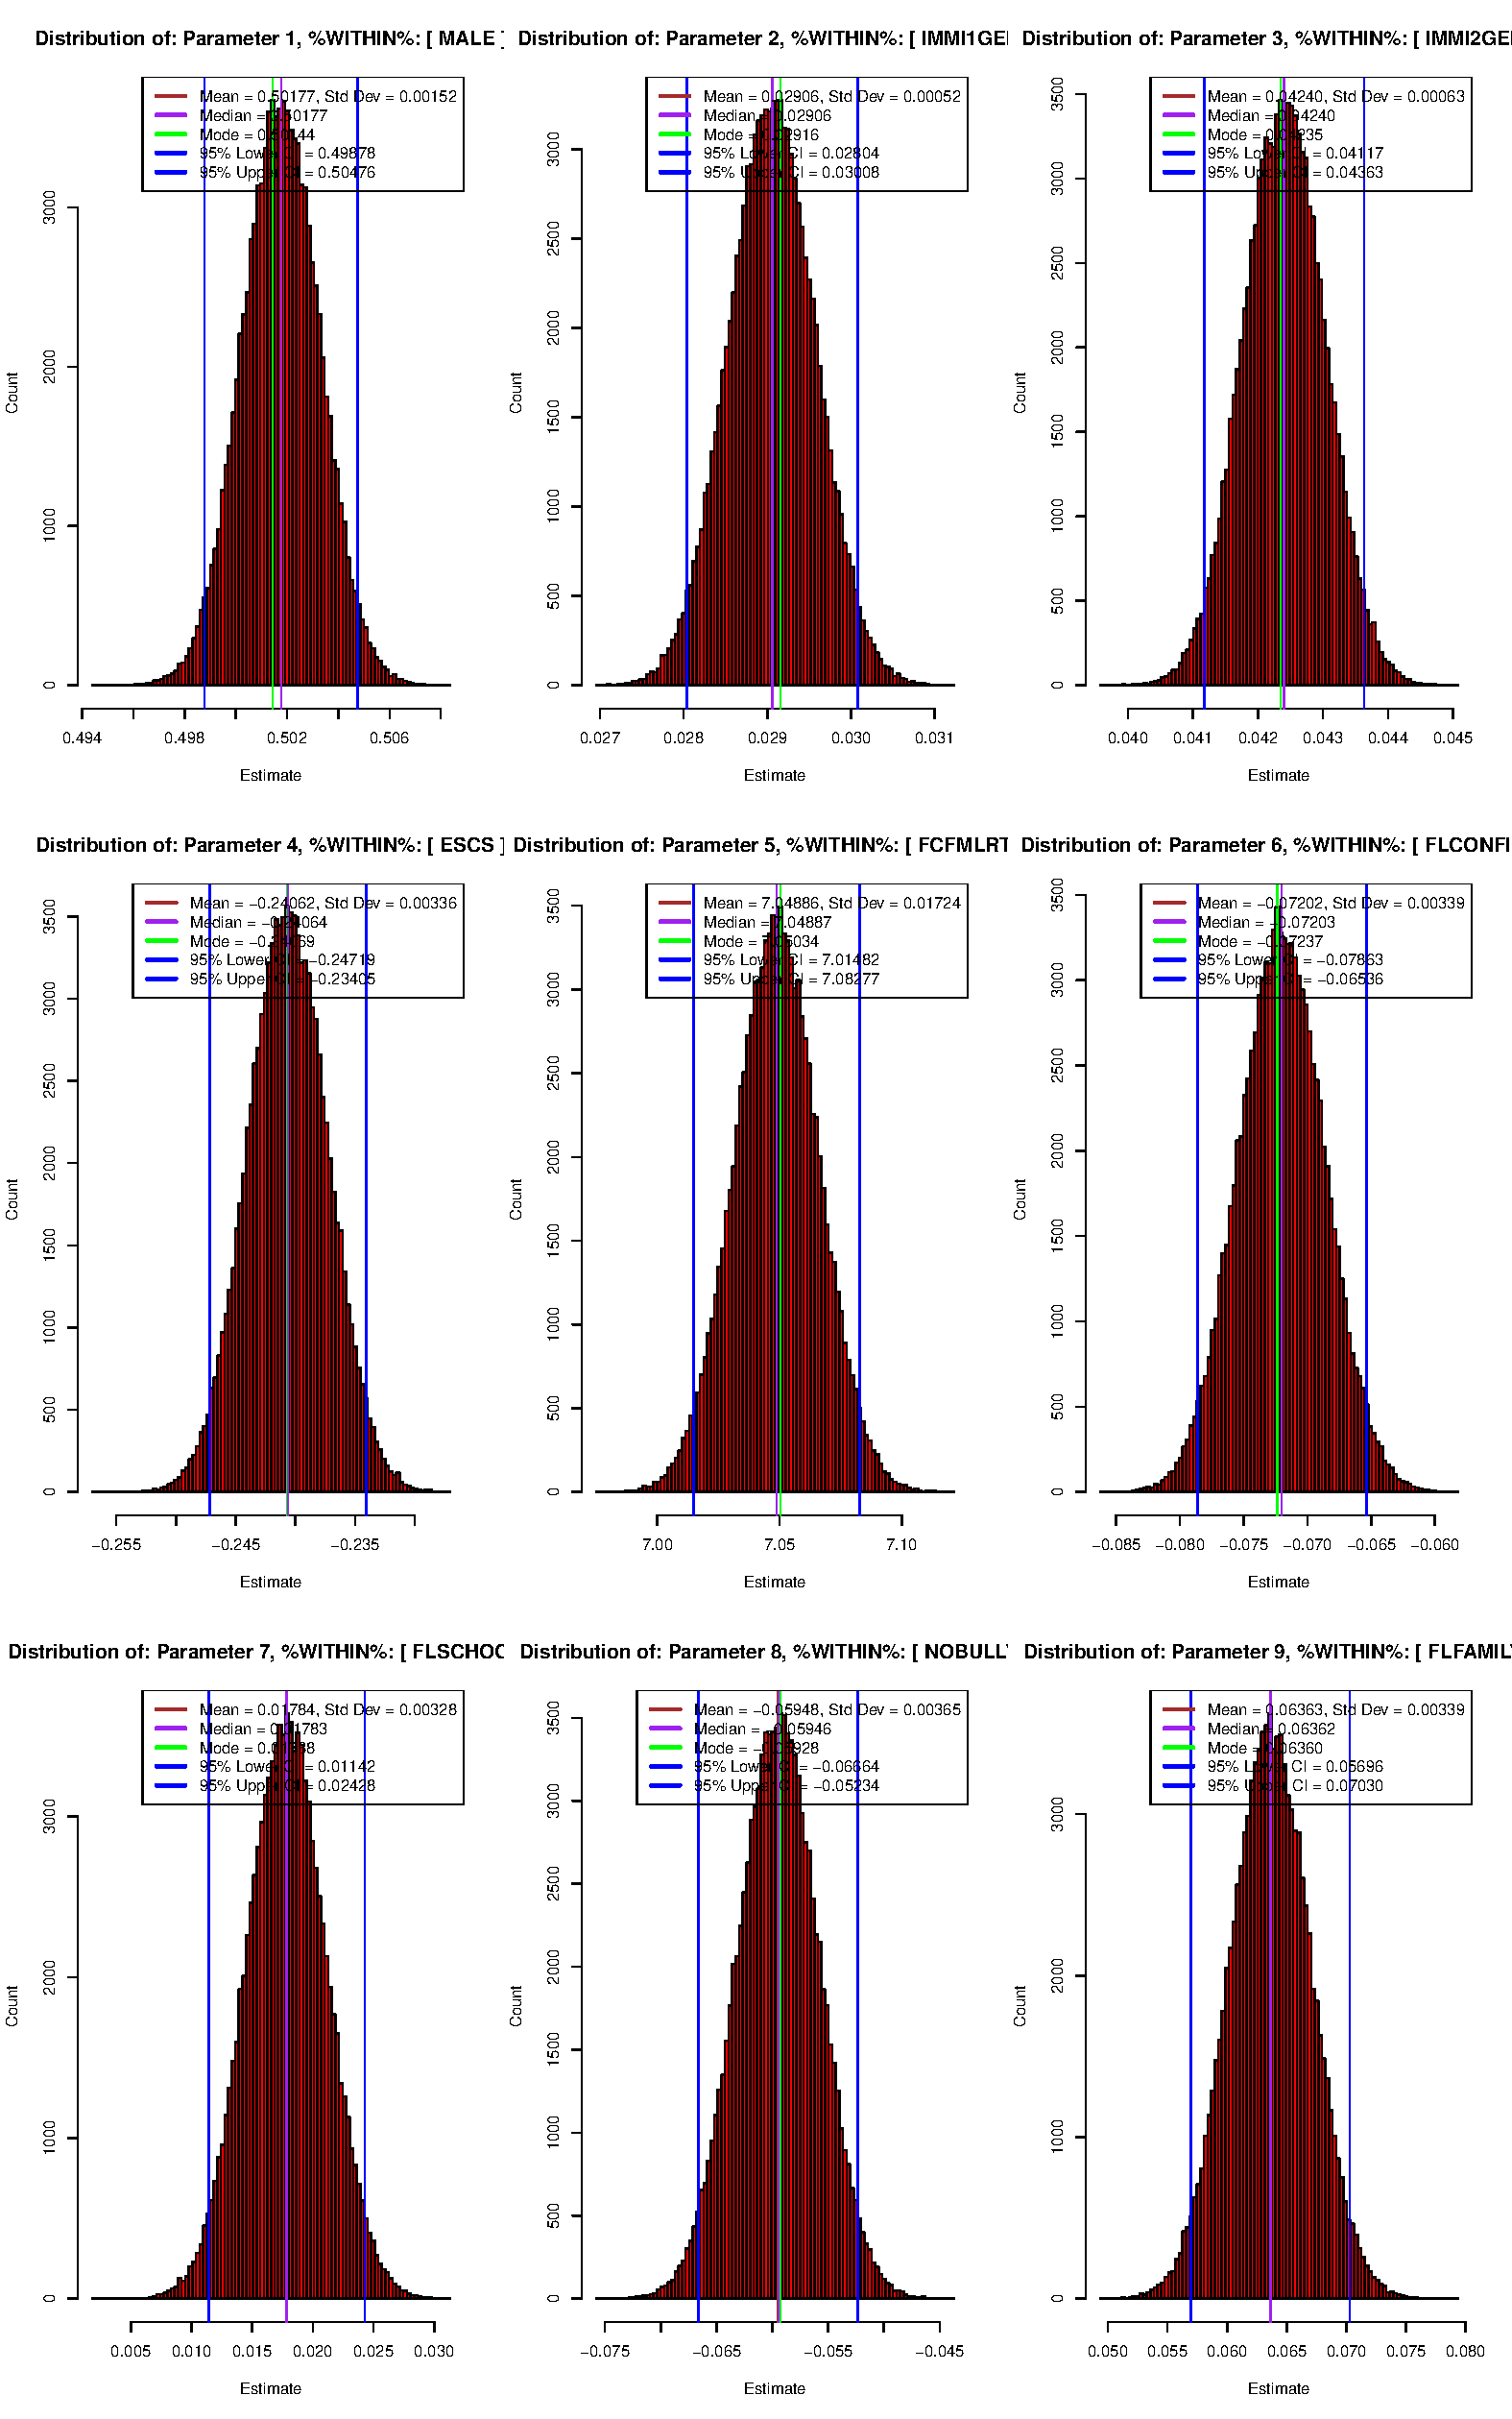
\includepdf[pages=-,width=\textwidth]{./Figures/MMI_diagnostic.pdf}

\subsection{MSEM Analysis Code}

\subsubsection{\cM Input}

\begin{MAEcode}
    \lstinputlisting[style=vscodeMplus]{./Mplus/M3/Two-structured.inp}
\end{MAEcode}

\subsubsection{Selected \cM Output}\label{sec:rsq}

\begin{MAEcode}
    \lstinputlisting[style=vscodeMplus_out,linerange={991-1007}]{./Mplus/M3/Two-structured.out}
\end{MAEcode}
